\chapter{Deep Learning Models for Fetal Pain Assessment}

In this chapter, we present some background topics recommended for a better understanding of our work and later explain the methodology that was used to conduct our experiments.

\section{Background}

In the task of image classification, traditional machine learning algorithms required hand-engineered features, like filters and descriptors, which were meant to extract information from the images to be used as an input for algorithms. These algorithms would then be trained to find patterns in these features capable of distinguishing between different classes.

Neural networks, on the other hand, have the advantage of being able to learn these features directly from the data, which makes the process of feature engineering a lot simpler and achieves better results in most cases. Furthermore, the recent advances in Deep Neural Networks have taken these capabilities to a new level. They not only win most of the competitions in the field but also achieve state of the art results in a wide range of real applications. One type of network that was responsible for these results is Convolutional Neural Networks (CNNs).

\subsection{Convolutional Neural Networks}

Convolutional Neural Networks are similar to traditional Neural Networks. They both have an input layer which receives the data, followed by hidden layers with numerous neurons with weights and biases capable of learning the characteristics of the data, and an output layer at the end which is responsible for classification. The main difference is that CNNs assume the input has some spatial relationship, which is a pattern present in images. Thus, knowledge of where pixels are located in reference to each other is preserved. CNNs are capable of extracting and capturing patterns from the images that would not have been possible if we used traditional networks. To extract these features, the networks uses two primary operations: convolution and pooling.

Convolutions are mathematical operations that act as learnable filters (also called kernels) to capture patterns in the images. These filters are usually small in terms of dimension, tipically 3x3 or 5x5 matrices. Each one of them convolves across the width and height of the input image and compute dot products with the pixels of the image, producing an activation map out of it. These activation maps, once learned, are able to detect features in the images, such as edges, corners, or color shifts. 

Pooling is another mathematical operation responsible for reducing the spatial size of the convolved feature. These series of transformations reduce the dimensionality of the data and makes it possible to process images of high resolution. 

As multiple convolutional and pooling layers are stacked, the network becomes able to detect more complex patterns that are composed of multiple inputs of different feature extractors in the first layers. By turning this activation maps back into images, we are able to see what kinds of features they are detecting, as demonstrated by \citep{ZeilerF14}. 

\subsection{Transfer Learning}

Transfer Learning is a technique commonly used in machine learning when a learning model that was originally developed for one task is then reused on a second related task. It comes from the assumption that what has been learned in one setting can be used to improve optimization in another setting. The idea behind is inspired by human behavior, as sometimes we can use expertise in solving one problem to solve another one.

Another motivation behind using transfer learning comes from the high computational cost necessary to train large deep neural networks for image classification. Since the number of parameters present in a CNN is very high, it requires a large amount of training data to tune the network for making precise predictions.

As an example, a commonly used dataset in the field, ImageNet \citep{DengDSLL009}, contains 1.2 million images and has 1000 categories to classify. Even with today's computational power, it still requires a significant amount of hours to be trained.

In this scenario, using transfer learning trough pre-trained networks arises as a solution. In this process, the weights and biases from a network trained in another task, are reused to train a new similar task.

Another reason for using transfer learning comes from the cases where we do not have enough data to train a CNN. \cite{CelonaBB19} highlights this is especially true in the medical field, as the acquisition costs are elevated, and it also involves a complicated setup for photographing, which makes it very common to have little annotated data.

\subsection{Data Augmentation}

Another solution that handles small datasets is data augmentation. It consists of applying transformations, such as geometric and color augmentations, for generating alternative images that derive from the original dataset.

For each input image in the dataset, a new image is generated that can be zoomed, shifted, mirrored, rotated, distorted, or have changes in its color, brightness, contrast. Hence, this technique increases the amount of data available for input. 

Having a large dataset is crucial for the performance of the deep learning models, but instead of starting with a large dataset of images, a more common scenario is to have a small amount of data available from the specific domain of research. This usually happens due to the high cost of collecting data, be it in terms of human labor or monetary resources. As mentioned in the previous section, this is mainly the case in the medical field. 

Another problem of small datasets is that problems trained on them are often over-fitted to the specific data available, which means they lack the power of generalization, as the dataset is not representative of the real world. 

In these cases, as discussed by \cite{abs-1712-04621}, data augmentation can act as a regularizer for preventing overfitting and also improve performance in imbalanced class problems.

% \subsection{Visual Explanations}

\section{Methodology}

Based on the techniques mentioned in the previous section, we have proposed a learning model for classifying between images of fetuses with facial expressions indicative of pain or not. In summary, our proposed pipeline consists of sampling the videos into frames, finding the images which contain a clear fetus face, and training a CNN in with the binary classification task of finding the presence of pain. In the following sections, we describe each of these steps.

\subsection{Image Sampling}

It is common to have a small number of data to work within the medical field, given the inherent difficulty of collecting it. In our case, especially, only a small percentage of pregnancies require intra-uterus intervention before birth, and thus fetal anesthesia is a relatively rare procedure. 

Thus, we ended up with 15 videos available. However, it is relatively common for studies in the field to also have a small N, as mentioned by \cite{ZamzmiPGKSA16}.

Since we had such a small number of videos, it was not possible to work with them directly. So, we decided to bring the data to another dimension, reducing the space from videos to images. In order to do this, we decided to sample the videos and capture frames at a rate of 2 seconds. 

With this process, we generated a total of 0000 images, but since the images were recorded from ultrasound machines, they depend on the calibration by the doctors to capture the exact section of the 3-D space where the fetus's face is clear. Because of this, it was common to find parts of the video where the face of the fetus was not visible and showed non-distinguishable parts.

As we had a significant number of images, and manual selection would be not only hard but also dependent on the observant, this became a problem.

To overcome this issue, we decided to use another neural network capable of detecting facial landmarks, like the nose, the mouth, and the eyes. The network we used was the Multi-task Cascaded Convolutional Networks (MTCNN) developed by \cite{ZhangZL016}, which identifies faces in images. It worked surprisingly well in our domain, even though the images had quite different characteristics.

With this process, we were able to filter out our dataset of images from 0000 to 0000 and be sure the images contained a clear face. The network returns a confidence number of which it found the face in the image, and we have used only confidences of over 95\%, which on manual inspection showed to be very reliable, with just six clear errors that were removed manually.

The position of the facial landmarks allowed us to crop the images around the face of the fetus, which is done just by adding padding to the places where they were. This process is achievable after we have the positions of the landmarks returned through the MTCNN, which also makes face alignment possible. This helps to discard images with blurred surroundings around the fetus, which contains non-distinguishable parts. 

At this point, manual selection was needed in other to separate the images back into the three groups. With the resting images, it was easy as all the frames were from resting positions. However, with the anesthesia and horn ones, we had to split the data between before and after the stimulus. This was not a complicated process as we knew precisely when the stimuli were applied, and a clear difference in the facial expression could be noted. After this step, we ended up with 0000 images, which had a visible face on it. Figure \ref{fig:cropping} shows an example of a cropped image.

\begin{figure}[h!tp]
    \centering
    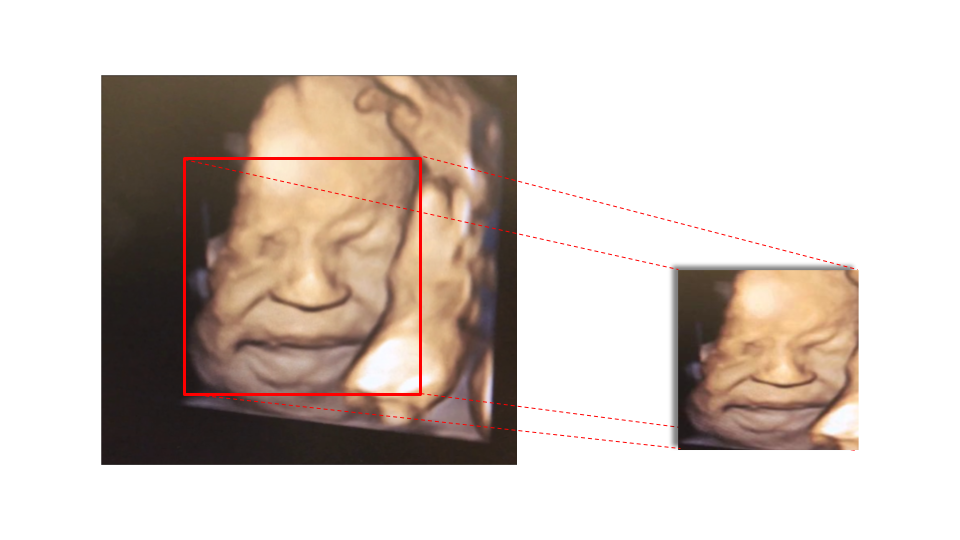
\includegraphics[width=.9\textwidth]{imgs/chap3_cropping.png}
    \caption{Image cropping with MTCNN}
    \label{fig:cropping}
\end{figure}

\subsection{Data Augmentation}

Even though we had increased the size of the dataset by turning the videos into images, it is still considered a relatively small dataset for deep learning models. To further augment our chances of succeeding, we have applied the use of data augmentation techniques to increase the variability of our data. The effectiveness of this technique has been demonstrated by \cite{abs-1712-04621} and is widely used in the field.

There is a wide variety of transformations possible for using data augmentation, and the most straightforward ones usually work very well. We have chosen the following:

\begin{itemize}
    \item Horizontal flip, which consists of mirroring the image horizontally. 
    \item Rotation, which consists in applying small rotations to the images.
    \item Zoom, which consists of zooming in the image.
    \item Lightning, which consists of changing the brightness and the contrast of the image.
    \item Warping, which consists of adding distortions to the image. 
\end{itemize}

All of these methods have a probability of being applied and can be used in combination with each other. Thus for each image, given the probability, a combination of these techniques would be applied. Some examples of these different combinations within the same image are shown in Figure \ref{fig:data_augmentation}.

\begin{figure}[h!tp]
    \centering
    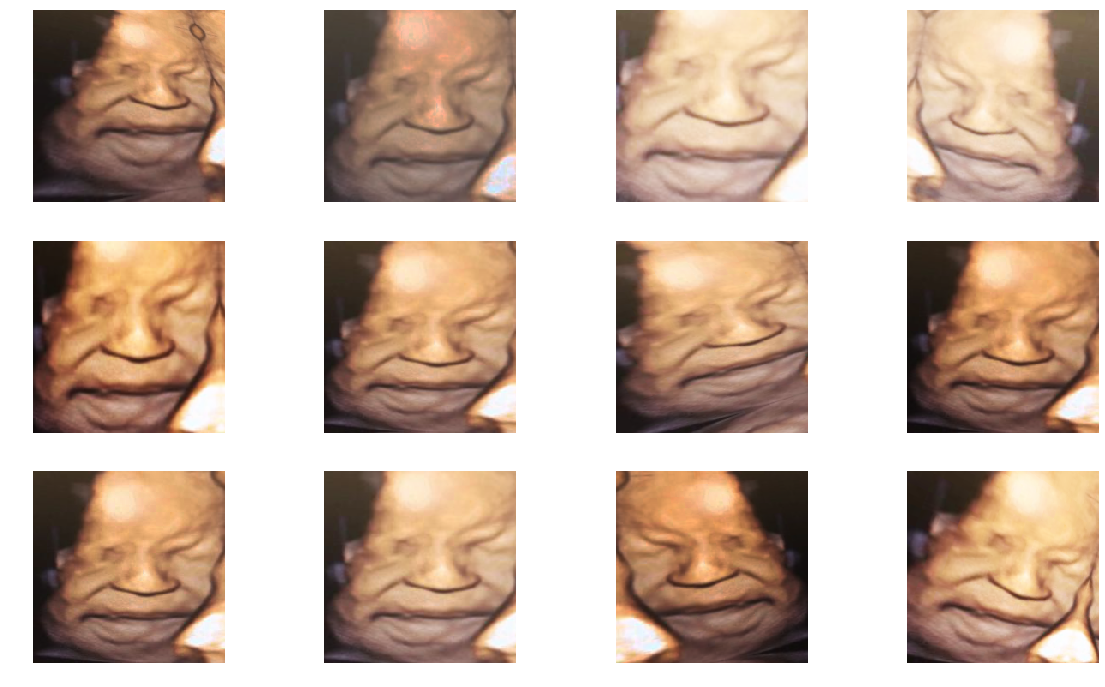
\includegraphics[width=.9\textwidth]{imgs/chap3_data_augmentation.png}
    \caption{The same image with different data augmentation applied}
    \label{fig:data_augmentation}
\end{figure}

To further experiment with this process, we have compared three levels of intensity in the changes, a smooth one, which does more subtle changes, a medium one, which intensifies a little bit and a more aggressive one, which applies substantial transformations to the images.

\subsection{Network Architecture and Transfer Learning}

The network used was VGG with a pre-trained model on VGG Face, developed by \cite{ParkhiVZ15}.



